\pagenumbering{arabic} 
\setcounter{page}{1}
\addcontentsline{toc}{part}{Building a Theremin}
\section{History and Theory}
\subsection{History}

The theremin was a product of research by the Russian government into proximity sensors and intelligence gathering. Lev Sergeivich Termen, known in Europe as Leon Theremin came across the apparatus' potential for sound production in October 1920. He showed it to Bolshevik leader Vladimir Lenin who dismissed the security value, but was incredibly impressed by the object as an instrument. He proposed that Theremin take it on a world tour to demonstrate the height of technology of the Soviet Union. This tour lasted until 1928 in Europe and, in 1929, he successfully patented the instrument in America. Despite the tour, the Theremin was not a commercial success until the mid 1930s and it fell into disuse after world war II when other electronic instruments came onto the market, such as the electric guitar, which had more immediate appeal though the sounds and relative easy of use. However, the theremin has remained a niche interest amongst electronic enthusiasts, such as Robert Moog, the inventor of the Moog Synthesiser and father of modern synthesizer technology.

The theremin was has had a variety of names, including the \ae therphone, thereminophone and termenvox and thereminvox. The final name was settled on after Theremin's death, using the Americanised version since that is where the patent was held at the time.

\subsection{Basic Theory}

The Theremin is an instrument which can be played without any physical contact from the user. This is certainly a contributing factor to its ongoing popularity amongst electronics enthusiasts such as Moog. 

The instrument uses two radio frequency oscillators to generate high frequency signals which are processed by a mixer. The mixer adds and subtracts the input signals and outputs a waveform which is chosen to be in the audible range, 20\,Hz to 20 000\,Hz. This method of converting high frequency signals down to lower frequency is known as heterodyning. One oscillator remains fixed whilst the other can be adjusted by a change in capacitance of the antenna connected to the instrument. The capacitor is formed by the user's hand, which is effectively a grounded plate, and the antenna. The resulting signal is amplified and played by a loud speaker.

This method of sound production allows for a wide, continuous range of frequencies, over the whole human audible range, and for different types of sound to be produced through the addition of post production effects being added to the waveform before being played. It also gives the instrument a unique sound that is sometimes desired in situations such as TV soundtracks.

\subsubsection{Generation - Oscillators}

The oscillators used come under the class of VCOs, voltage control oscillators, as the input voltage is directly proportional to the frequency of the signal generated. 

\begin{wrapfigure}[10]{r}{0.4\textwidth}
  \begin{center}
    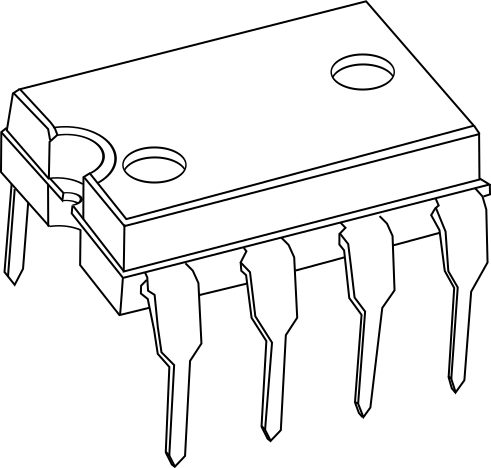
\includegraphics[width=0.3\textwidth]{report_img/ic}
  \end{center}
  \caption{A 555 timer integrated circuit VCO for use in bread board electronics.}
  \label{fig:timer ic}
\end{wrapfigure}

The VCOs are given an input voltage and output a series of pulses with a high time and low time determined by their governing equations. These equations are calculated by the manufacturers and vary between models, specific cases are discussed in sections~\ref{sec:555},~\ref{sec:4046} and~\ref{sec:7555}. This high-low nature means that the output signal is a close approximation to a square wave. A perfect sound wave is sinusoidal so this is not the ideal case, however, later stages in signal processing lead to the shape changing slightly and the difference in audible quality due to the wave not being sinusoidal is slight.

The VCOs are complete components supplied in the form of an monolithic integrated circuit, called an IC. They comprise a variety of components that shall be treated as a complete separate entity. These ICs are included in the circuit to perform a particular action, the inner workings will not be considered for this report.

\subsubsection{Control - Capacitor}
The capacitor is a simple parallel plate capacitor, one plate formed by the antenna, connected to the circuit, the other being the user's hand, or any other body part or other conducting object, that is near the first plate. The user is effectively grounded so the capacitor is connected once to the circuit and once to ground, as shown in figure~\ref{fig:capacitor}. The capacitor equation is given by,

\begin{figure}[htbp]
  \begin{center}
    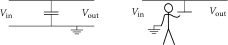
\includegraphics[scale=1.2]{report_img/plate_capacitor}
    \caption{A capacitor is used to control the sound produced by the circuit. When in the theremin, the capacitor is replaced by an antenna and a separate plate formed of the user's hand.}
    \label{fig:capacitor}
  \end{center}
\end{figure}

When the user moves closer to the plate, the capacitance decreases and, likewise, the capacitance increases when the user moves away. Also the area of plate, i.e.\ the size of the user's hand, will change the capacitance, in accordance with the capacitor equation, equation~(\ref{eqn:capacitor}), which gives another mode of control over the sound produced.
\begin{align}
  C &= \frac{k\varepsilon_0 A}{d}, \label{eqn:capacitor}
\end{align}
where,
\begin{itemize}
  \item $k$ is the relative permittivity of the dielectric material between the plates, in this case air which has $k=1$,
  \item $\varepsilon_0$ is the permittivity of free space, $\varepsilon_0 = 8.85 \times 10^{-12} \text{Fm}^{-1}$,
  \item $A$ is the area of the plates and
  \item $d$ is the separation of the two plates.
\end{itemize}

\newpage 
